% Created by tikzDevice version 0.12.6 on 2024-04-08 15:44:17
% !TEX encoding = UTF-8 Unicode
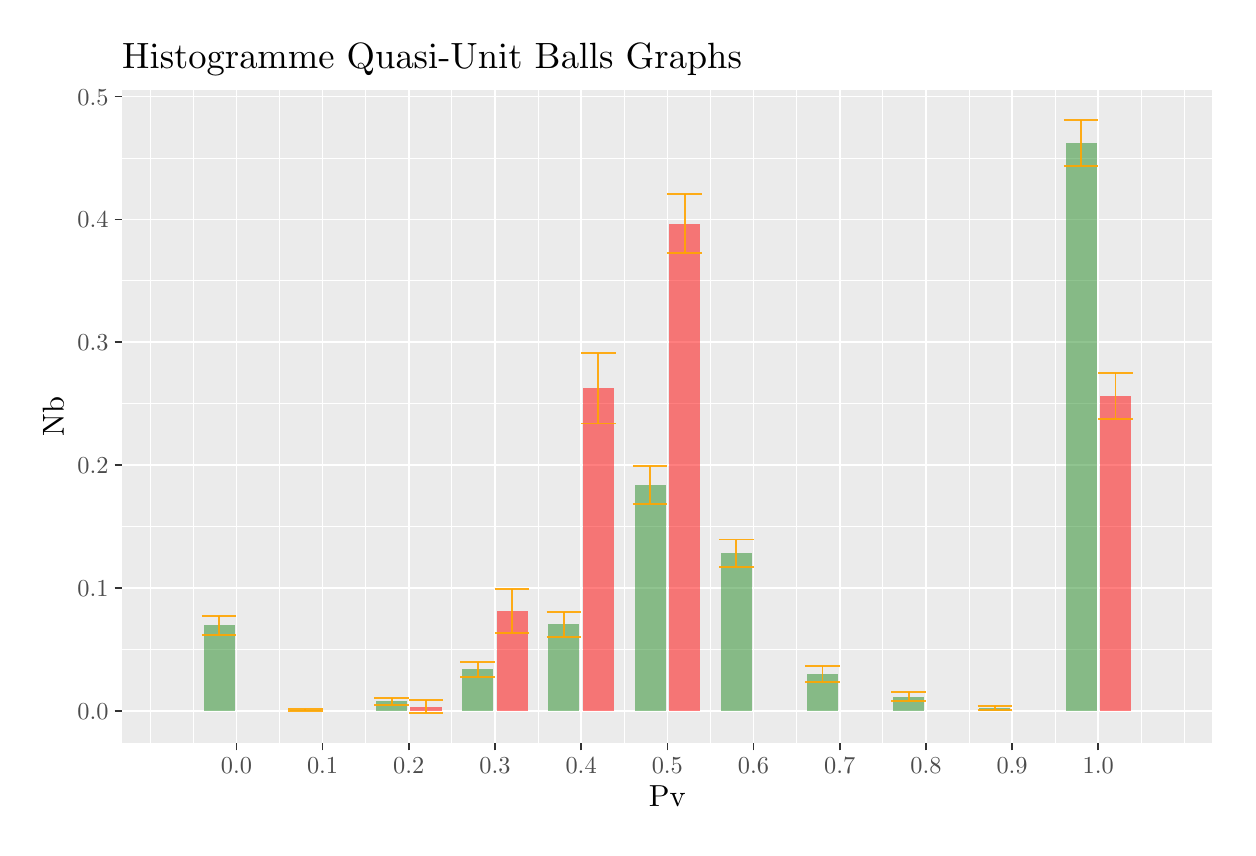
\begin{tikzpicture}[x=1pt,y=1pt]
\definecolor{fillColor}{RGB}{255,255,255}
\path[use as bounding box,fill=fillColor,fill opacity=0.00] (0,0) rectangle (433.62,289.08);
\begin{scope}
\path[clip] (  0.00,  0.00) rectangle (433.62,289.08);
\definecolor{drawColor}{RGB}{255,255,255}
\definecolor{fillColor}{RGB}{255,255,255}

\path[draw=drawColor,line width= 0.6pt,line join=round,line cap=round,fill=fillColor] (  0.00,  0.00) rectangle (433.62,289.08);
\end{scope}
\begin{scope}
\path[clip] ( 34.16, 30.69) rectangle (428.12,266.42);
\definecolor{fillColor}{gray}{0.92}

\path[fill=fillColor] ( 34.16, 30.69) rectangle (428.12,266.42);
\definecolor{drawColor}{RGB}{255,255,255}

\path[draw=drawColor,line width= 0.3pt,line join=round] ( 34.16, 64.45) --
	(428.12, 64.45);

\path[draw=drawColor,line width= 0.3pt,line join=round] ( 34.16,108.83) --
	(428.12,108.83);

\path[draw=drawColor,line width= 0.3pt,line join=round] ( 34.16,153.21) --
	(428.12,153.21);

\path[draw=drawColor,line width= 0.3pt,line join=round] ( 34.16,197.59) --
	(428.12,197.59);

\path[draw=drawColor,line width= 0.3pt,line join=round] ( 34.16,241.97) --
	(428.12,241.97);

\path[draw=drawColor,line width= 0.3pt,line join=round] ( 44.28, 30.69) --
	( 44.28,266.42);

\path[draw=drawColor,line width= 0.3pt,line join=round] ( 59.85, 30.69) --
	( 59.85,266.42);

\path[draw=drawColor,line width= 0.3pt,line join=round] ( 90.99, 30.69) --
	( 90.99,266.42);

\path[draw=drawColor,line width= 0.3pt,line join=round] (122.14, 30.69) --
	(122.14,266.42);

\path[draw=drawColor,line width= 0.3pt,line join=round] (153.28, 30.69) --
	(153.28,266.42);

\path[draw=drawColor,line width= 0.3pt,line join=round] (184.42, 30.69) --
	(184.42,266.42);

\path[draw=drawColor,line width= 0.3pt,line join=round] (215.57, 30.69) --
	(215.57,266.42);

\path[draw=drawColor,line width= 0.3pt,line join=round] (246.71, 30.69) --
	(246.71,266.42);

\path[draw=drawColor,line width= 0.3pt,line join=round] (277.85, 30.69) --
	(277.85,266.42);

\path[draw=drawColor,line width= 0.3pt,line join=round] (309.00, 30.69) --
	(309.00,266.42);

\path[draw=drawColor,line width= 0.3pt,line join=round] (340.14, 30.69) --
	(340.14,266.42);

\path[draw=drawColor,line width= 0.3pt,line join=round] (371.28, 30.69) --
	(371.28,266.42);

\path[draw=drawColor,line width= 0.3pt,line join=round] (402.43, 30.69) --
	(402.43,266.42);

\path[draw=drawColor,line width= 0.3pt,line join=round] (418.00, 30.69) --
	(418.00,266.42);

\path[draw=drawColor,line width= 0.6pt,line join=round] ( 34.16, 42.26) --
	(428.12, 42.26);

\path[draw=drawColor,line width= 0.6pt,line join=round] ( 34.16, 86.64) --
	(428.12, 86.64);

\path[draw=drawColor,line width= 0.6pt,line join=round] ( 34.16,131.02) --
	(428.12,131.02);

\path[draw=drawColor,line width= 0.6pt,line join=round] ( 34.16,175.40) --
	(428.12,175.40);

\path[draw=drawColor,line width= 0.6pt,line join=round] ( 34.16,219.78) --
	(428.12,219.78);

\path[draw=drawColor,line width= 0.6pt,line join=round] ( 34.16,264.16) --
	(428.12,264.16);

\path[draw=drawColor,line width= 0.6pt,line join=round] ( 75.42, 30.69) --
	( 75.42,266.42);

\path[draw=drawColor,line width= 0.6pt,line join=round] (106.56, 30.69) --
	(106.56,266.42);

\path[draw=drawColor,line width= 0.6pt,line join=round] (137.71, 30.69) --
	(137.71,266.42);

\path[draw=drawColor,line width= 0.6pt,line join=round] (168.85, 30.69) --
	(168.85,266.42);

\path[draw=drawColor,line width= 0.6pt,line join=round] (199.99, 30.69) --
	(199.99,266.42);

\path[draw=drawColor,line width= 0.6pt,line join=round] (231.14, 30.69) --
	(231.14,266.42);

\path[draw=drawColor,line width= 0.6pt,line join=round] (262.28, 30.69) --
	(262.28,266.42);

\path[draw=drawColor,line width= 0.6pt,line join=round] (293.42, 30.69) --
	(293.42,266.42);

\path[draw=drawColor,line width= 0.6pt,line join=round] (324.57, 30.69) --
	(324.57,266.42);

\path[draw=drawColor,line width= 0.6pt,line join=round] (355.71, 30.69) --
	(355.71,266.42);

\path[draw=drawColor,line width= 0.6pt,line join=round] (386.86, 30.69) --
	(386.86,266.42);
\definecolor{fillColor}{RGB}{34,139,34}

\path[fill=fillColor,fill opacity=0.50] ( 63.59, 42.26) rectangle ( 74.80, 73.08);

\path[fill=fillColor,fill opacity=0.50] ( 94.73, 42.26) rectangle (105.94, 42.60);

\path[fill=fillColor,fill opacity=0.50] (125.87, 42.26) rectangle (137.09, 45.63);

\path[fill=fillColor,fill opacity=0.50] (157.02, 42.26) rectangle (168.23, 57.21);

\path[fill=fillColor,fill opacity=0.50] (188.16, 42.26) rectangle (199.37, 73.43);

\path[fill=fillColor,fill opacity=0.50] (219.30, 42.26) rectangle (230.52,123.82);

\path[fill=fillColor,fill opacity=0.50] (250.45, 42.26) rectangle (261.66, 99.20);

\path[fill=fillColor,fill opacity=0.50] (281.59, 42.26) rectangle (292.80, 55.57);

\path[fill=fillColor,fill opacity=0.50] (312.73, 42.26) rectangle (323.95, 47.38);

\path[fill=fillColor,fill opacity=0.50] (343.88, 42.26) rectangle (355.09, 43.38);

\path[fill=fillColor,fill opacity=0.50] (375.02, 42.26) rectangle (386.23,247.34);
\definecolor{fillColor}{RGB}{255,0,0}

\path[fill=fillColor,fill opacity=0.50] (138.33, 42.26) rectangle (149.54, 43.76);

\path[fill=fillColor,fill opacity=0.50] (169.47, 42.26) rectangle (180.69, 78.30);

\path[fill=fillColor,fill opacity=0.50] (200.62, 42.26) rectangle (211.83,158.81);

\path[fill=fillColor,fill opacity=0.50] (231.76, 42.26) rectangle (242.97,218.20);

\path[fill=fillColor,fill opacity=0.50] (387.48, 42.26) rectangle (398.69,156.02);
\definecolor{drawColor}{RGB}{255,165,0}

\path[draw=drawColor,draw opacity=0.90,line width= 0.7pt,line join=round] ( 62.96, 76.61) --
	( 75.42, 76.61);

\path[draw=drawColor,draw opacity=0.90,line width= 0.7pt,line join=round] ( 69.19, 76.61) --
	( 69.19, 69.55);

\path[draw=drawColor,draw opacity=0.90,line width= 0.7pt,line join=round] ( 62.96, 69.55) --
	( 75.42, 69.55);

\path[draw=drawColor,draw opacity=0.90,line width= 0.7pt,line join=round] ( 94.11, 43.01) --
	(106.56, 43.01);

\path[draw=drawColor,draw opacity=0.90,line width= 0.7pt,line join=round] (100.34, 43.01) --
	(100.34, 42.19);

\path[draw=drawColor,draw opacity=0.90,line width= 0.7pt,line join=round] ( 94.11, 42.19) --
	(106.56, 42.19);

\path[draw=drawColor,draw opacity=0.90,line width= 0.7pt,line join=round] (125.25, 47.01) --
	(137.71, 47.01);

\path[draw=drawColor,draw opacity=0.90,line width= 0.7pt,line join=round] (131.48, 47.01) --
	(131.48, 44.25);

\path[draw=drawColor,draw opacity=0.90,line width= 0.7pt,line join=round] (125.25, 44.25) --
	(137.71, 44.25);

\path[draw=drawColor,draw opacity=0.90,line width= 0.7pt,line join=round] (156.39, 59.90) --
	(168.85, 59.90);

\path[draw=drawColor,draw opacity=0.90,line width= 0.7pt,line join=round] (162.62, 59.90) --
	(162.62, 54.53);

\path[draw=drawColor,draw opacity=0.90,line width= 0.7pt,line join=round] (156.39, 54.53) --
	(168.85, 54.53);

\path[draw=drawColor,draw opacity=0.90,line width= 0.7pt,line join=round] (187.54, 77.99) --
	(199.99, 77.99);

\path[draw=drawColor,draw opacity=0.90,line width= 0.7pt,line join=round] (193.77, 77.99) --
	(193.77, 68.88);

\path[draw=drawColor,draw opacity=0.90,line width= 0.7pt,line join=round] (187.54, 68.88) --
	(199.99, 68.88);

\path[draw=drawColor,draw opacity=0.90,line width= 0.7pt,line join=round] (218.68,130.63) --
	(231.14,130.63);

\path[draw=drawColor,draw opacity=0.90,line width= 0.7pt,line join=round] (224.91,130.63) --
	(224.91,117.01);

\path[draw=drawColor,draw opacity=0.90,line width= 0.7pt,line join=round] (218.68,117.01) --
	(231.14,117.01);

\path[draw=drawColor,draw opacity=0.90,line width= 0.7pt,line join=round] (249.82,104.12) --
	(262.28,104.12);

\path[draw=drawColor,draw opacity=0.90,line width= 0.7pt,line join=round] (256.05,104.12) --
	(256.05, 94.29);

\path[draw=drawColor,draw opacity=0.90,line width= 0.7pt,line join=round] (249.82, 94.29) --
	(262.28, 94.29);

\path[draw=drawColor,draw opacity=0.90,line width= 0.7pt,line join=round] (280.97, 58.35) --
	(293.42, 58.35);

\path[draw=drawColor,draw opacity=0.90,line width= 0.7pt,line join=round] (287.20, 58.35) --
	(287.20, 52.78);

\path[draw=drawColor,draw opacity=0.90,line width= 0.7pt,line join=round] (280.97, 52.78) --
	(293.42, 52.78);

\path[draw=drawColor,draw opacity=0.90,line width= 0.7pt,line join=round] (312.11, 48.87) --
	(324.57, 48.87);

\path[draw=drawColor,draw opacity=0.90,line width= 0.7pt,line join=round] (318.34, 48.87) --
	(318.34, 45.89);

\path[draw=drawColor,draw opacity=0.90,line width= 0.7pt,line join=round] (312.11, 45.89) --
	(324.57, 45.89);

\path[draw=drawColor,draw opacity=0.90,line width= 0.7pt,line join=round] (343.25, 44.10) --
	(355.71, 44.10);

\path[draw=drawColor,draw opacity=0.90,line width= 0.7pt,line join=round] (349.48, 44.10) --
	(349.48, 42.66);

\path[draw=drawColor,draw opacity=0.90,line width= 0.7pt,line join=round] (343.25, 42.66) --
	(355.71, 42.66);

\path[draw=drawColor,draw opacity=0.90,line width= 0.7pt,line join=round] (374.40,255.71) --
	(386.86,255.71);

\path[draw=drawColor,draw opacity=0.90,line width= 0.7pt,line join=round] (380.63,255.71) --
	(380.63,238.98);

\path[draw=drawColor,draw opacity=0.90,line width= 0.7pt,line join=round] (374.40,238.98) --
	(386.86,238.98);

\path[draw=drawColor,draw opacity=0.90,line width= 0.7pt,line join=round] (137.71, 46.12) --
	(150.17, 46.12);

\path[draw=drawColor,draw opacity=0.90,line width= 0.7pt,line join=round] (143.94, 46.12) --
	(143.94, 41.40);

\path[draw=drawColor,draw opacity=0.90,line width= 0.7pt,line join=round] (137.71, 41.40) --
	(150.17, 41.40);

\path[draw=drawColor,draw opacity=0.90,line width= 0.7pt,line join=round] (168.85, 86.27) --
	(181.31, 86.27);

\path[draw=drawColor,draw opacity=0.90,line width= 0.7pt,line join=round] (175.08, 86.27) --
	(175.08, 70.33);

\path[draw=drawColor,draw opacity=0.90,line width= 0.7pt,line join=round] (168.85, 70.33) --
	(181.31, 70.33);

\path[draw=drawColor,draw opacity=0.90,line width= 0.7pt,line join=round] (199.99,171.58) --
	(212.45,171.58);

\path[draw=drawColor,draw opacity=0.90,line width= 0.7pt,line join=round] (206.22,171.58) --
	(206.22,146.04);

\path[draw=drawColor,draw opacity=0.90,line width= 0.7pt,line join=round] (199.99,146.04) --
	(212.45,146.04);

\path[draw=drawColor,draw opacity=0.90,line width= 0.7pt,line join=round] (231.14,228.86) --
	(243.60,228.86);

\path[draw=drawColor,draw opacity=0.90,line width= 0.7pt,line join=round] (237.37,228.86) --
	(237.37,207.54);

\path[draw=drawColor,draw opacity=0.90,line width= 0.7pt,line join=round] (231.14,207.54) --
	(243.60,207.54);

\path[draw=drawColor,draw opacity=0.90,line width= 0.7pt,line join=round] (386.86,164.22) --
	(399.31,164.22);

\path[draw=drawColor,draw opacity=0.90,line width= 0.7pt,line join=round] (393.08,164.22) --
	(393.08,147.81);

\path[draw=drawColor,draw opacity=0.90,line width= 0.7pt,line join=round] (386.86,147.81) --
	(399.31,147.81);
\end{scope}
\begin{scope}
\path[clip] (  0.00,  0.00) rectangle (433.62,289.08);
\definecolor{drawColor}{gray}{0.30}

\node[text=drawColor,anchor=base east,inner sep=0pt, outer sep=0pt, scale=  0.88] at ( 29.21, 39.23) {0.0};

\node[text=drawColor,anchor=base east,inner sep=0pt, outer sep=0pt, scale=  0.88] at ( 29.21, 83.61) {0.1};

\node[text=drawColor,anchor=base east,inner sep=0pt, outer sep=0pt, scale=  0.88] at ( 29.21,127.99) {0.2};

\node[text=drawColor,anchor=base east,inner sep=0pt, outer sep=0pt, scale=  0.88] at ( 29.21,172.37) {0.3};

\node[text=drawColor,anchor=base east,inner sep=0pt, outer sep=0pt, scale=  0.88] at ( 29.21,216.75) {0.4};

\node[text=drawColor,anchor=base east,inner sep=0pt, outer sep=0pt, scale=  0.88] at ( 29.21,261.13) {0.5};
\end{scope}
\begin{scope}
\path[clip] (  0.00,  0.00) rectangle (433.62,289.08);
\definecolor{drawColor}{gray}{0.20}

\path[draw=drawColor,line width= 0.6pt,line join=round] ( 31.41, 42.26) --
	( 34.16, 42.26);

\path[draw=drawColor,line width= 0.6pt,line join=round] ( 31.41, 86.64) --
	( 34.16, 86.64);

\path[draw=drawColor,line width= 0.6pt,line join=round] ( 31.41,131.02) --
	( 34.16,131.02);

\path[draw=drawColor,line width= 0.6pt,line join=round] ( 31.41,175.40) --
	( 34.16,175.40);

\path[draw=drawColor,line width= 0.6pt,line join=round] ( 31.41,219.78) --
	( 34.16,219.78);

\path[draw=drawColor,line width= 0.6pt,line join=round] ( 31.41,264.16) --
	( 34.16,264.16);
\end{scope}
\begin{scope}
\path[clip] (  0.00,  0.00) rectangle (433.62,289.08);
\definecolor{drawColor}{gray}{0.20}

\path[draw=drawColor,line width= 0.6pt,line join=round] ( 75.42, 27.94) --
	( 75.42, 30.69);

\path[draw=drawColor,line width= 0.6pt,line join=round] (106.56, 27.94) --
	(106.56, 30.69);

\path[draw=drawColor,line width= 0.6pt,line join=round] (137.71, 27.94) --
	(137.71, 30.69);

\path[draw=drawColor,line width= 0.6pt,line join=round] (168.85, 27.94) --
	(168.85, 30.69);

\path[draw=drawColor,line width= 0.6pt,line join=round] (199.99, 27.94) --
	(199.99, 30.69);

\path[draw=drawColor,line width= 0.6pt,line join=round] (231.14, 27.94) --
	(231.14, 30.69);

\path[draw=drawColor,line width= 0.6pt,line join=round] (262.28, 27.94) --
	(262.28, 30.69);

\path[draw=drawColor,line width= 0.6pt,line join=round] (293.42, 27.94) --
	(293.42, 30.69);

\path[draw=drawColor,line width= 0.6pt,line join=round] (324.57, 27.94) --
	(324.57, 30.69);

\path[draw=drawColor,line width= 0.6pt,line join=round] (355.71, 27.94) --
	(355.71, 30.69);

\path[draw=drawColor,line width= 0.6pt,line join=round] (386.86, 27.94) --
	(386.86, 30.69);
\end{scope}
\begin{scope}
\path[clip] (  0.00,  0.00) rectangle (433.62,289.08);
\definecolor{drawColor}{gray}{0.30}

\node[text=drawColor,anchor=base,inner sep=0pt, outer sep=0pt, scale=  0.88] at ( 75.42, 19.68) {0.0};

\node[text=drawColor,anchor=base,inner sep=0pt, outer sep=0pt, scale=  0.88] at (106.56, 19.68) {0.1};

\node[text=drawColor,anchor=base,inner sep=0pt, outer sep=0pt, scale=  0.88] at (137.71, 19.68) {0.2};

\node[text=drawColor,anchor=base,inner sep=0pt, outer sep=0pt, scale=  0.88] at (168.85, 19.68) {0.3};

\node[text=drawColor,anchor=base,inner sep=0pt, outer sep=0pt, scale=  0.88] at (199.99, 19.68) {0.4};

\node[text=drawColor,anchor=base,inner sep=0pt, outer sep=0pt, scale=  0.88] at (231.14, 19.68) {0.5};

\node[text=drawColor,anchor=base,inner sep=0pt, outer sep=0pt, scale=  0.88] at (262.28, 19.68) {0.6};

\node[text=drawColor,anchor=base,inner sep=0pt, outer sep=0pt, scale=  0.88] at (293.42, 19.68) {0.7};

\node[text=drawColor,anchor=base,inner sep=0pt, outer sep=0pt, scale=  0.88] at (324.57, 19.68) {0.8};

\node[text=drawColor,anchor=base,inner sep=0pt, outer sep=0pt, scale=  0.88] at (355.71, 19.68) {0.9};

\node[text=drawColor,anchor=base,inner sep=0pt, outer sep=0pt, scale=  0.88] at (386.86, 19.68) {1.0};
\end{scope}
\begin{scope}
\path[clip] (  0.00,  0.00) rectangle (433.62,289.08);
\definecolor{drawColor}{RGB}{0,0,0}

\node[text=drawColor,anchor=base,inner sep=0pt, outer sep=0pt, scale=  1.10] at (231.14,  7.64) {Pv};
\end{scope}
\begin{scope}
\path[clip] (  0.00,  0.00) rectangle (433.62,289.08);
\definecolor{drawColor}{RGB}{0,0,0}

\node[text=drawColor,rotate= 90.00,anchor=base,inner sep=0pt, outer sep=0pt, scale=  1.10] at ( 13.08,148.55) {Nb};
\end{scope}
\begin{scope}
\path[clip] (  0.00,  0.00) rectangle (433.62,289.08);
\definecolor{drawColor}{RGB}{0,0,0}

\node[text=drawColor,anchor=base west,inner sep=0pt, outer sep=0pt, scale=  1.32] at ( 34.16,274.49) {Histogramme Quasi-Unit Balls Graphs};
\end{scope}
\end{tikzpicture}
